\documentclass[11pt]{article}
\usepackage{acl2014}
\usepackage{times}
\usepackage{url}
\usepackage{latexsym}
\usepackage{graphicx}
\usepackage{float}
\title{Coconut palms and hand palms: improving similarity ranking by word sense disambiguation}

\author{Anouk Visser \\
  {\tt anouk.visser@me.com} \\\And
  R\'emi de Zoeten \\
  {\tt remi.de.z@gmail.com} \\}

\date{}

\begin{document}
\maketitle
\begin{abstract}


\end{abstract}

\section{Introduction}

\section{Related Work}
The task of word sense disambiguation is to assign the correct sense to an ambiguous word, whereas word sense discrimination is the task of finding the different senses a word might have \cite{old}. The importance of using co-occurrences for determining the correct sense of a word is already emphasized in \cite{relatedness} in which the authors propose a method for word sense disambiguation using co-occurrences. More specifically, the authors propose a simple score expressing the relatedness between two words:
\begin{equation}\label{r}r(x, y) = \frac{f_{xy}}{f_x+f_y - f_{xy}}\end{equation}
where $f_{xy}$ denotes the frequency of $x$ and $y$ occurring together and $f_x$ and $f_y$ denote the frequency of $x$, respectively $y$. 
In the past years a lot of different methods for word sense disambiguation have been proposed that can be classified as supervised, knowledge-based or unsupervised methods\cite{survey}. Unsupervised WSD mainly focus on word sense discrimination, the majority of unsupervised word sense discrimination methods use clustering on, for example, context vectors or relatedness vectors. An example of an unsupervised method that uses clustering on both first order context vectors and second order context vectors can be found in \cite{clustering}. Another example of unsupervised word sense discrimination is given in \cite{latent} where the authors use the intuition that the meaning of a word can be represented as a distribution over a set of latent senses.


Recently \cite{word2vec} have released tools for efficiently computing word vectors that capture syntactic and semantic information. The distance between these vectors can be used for identifying linguistic regularities \cite{regularities} and a number of other applications such as word sense discrimination through clustering these word vectors. However, word vector representations suffer from the problem that words may have a number of different meanings that cannot be captured in a single representation. \cite{multi} propose a solution to this problem by representing a word's meaning by a set of sense specific word vectors which are discovered by clustering the contexts in which the word appears. For every context cluster, the authors compute an average vector that can be used to determine the similarity between two words (either in context or isolated). A drawback of this method is that it is required to know the number of senses in advance. \cite{global} build upon this work by introducing a new neural network architecture that learns word vectors by also incorporating the global context of a word and can lean multiple vectors for a single word. In addition to this, they present a new dataset of pairs of words in contexts annotated with similarity judgements by human annotators. 

\begin{table*}
    \begin{tabular}{|p{5cm}|p{5cm}|p{5cm}|}
    \hline
    \textbf{bat} & \textbf{course} & \textbf{bank}                                                                                                                                \\ \hline
    batter, superfamilies, inning, ye, ball, batman, cave, ruth, pitch, slug, hitter, base, plate, flies, mammal    & hole, student, action, educate, online, learn, studies, disc, teach, meal, hungarian, university, employee, lecture, play & reserve, imf, central, account, money, finance, european, deposit, sweden, invest, intern, cccc, palestinian, note, economic, tower \\ \hline
    average, hit, cricket, baseball, out, funnel, casey, score, rabies, runner, myotis, ab, statist, league, pollin & golf, caddie, require, taught, offer, historic, distance, college, typic, qualify, event, year, decide, entire, business  & gaza, strip, monetary, financial, river, fund, feder, currency, settlement, england, loan, sector, israel, jordan, isra             \\\hline
    \end{tabular}
    \caption{Table showing the 15 most related words in the two sense clusters (clustered with $k=2$) of the words \textit{bat}, \textit{bank} and \textit{course}. For bat we observe a lot of noise, however the majority of words that describe bat-as-in animal are in the first cluster (superfamilies, batman, cave, flies, mammal). The first sense of course is focussed towards learning (student, educate, online) as well as meals, the second sense also contains the words golf, caddie and distance which refer to course-as-in golf. Finally, for bank we find that the second cluster contains word referring to river (river, settlement, strip) as well as words referring to the middle east (gaza, israel, jordan). The first cluster is more focussed towards bank as a financial institution. }
\label{coconutres}

\end{table*}

\section{Training data}
For model training data we used the \textit{enwiki8} dataset\footnote{http://mattmahoney.net/dc/textdata.html} corpus. For our purposes we filtered the corpus to only keep the words in the following Part-Of-Speech categories: Nouns, Verbs, Adjectives and Adverbs as is common in word sense disambiguation and discrimination systems \cite{survey}. Furthermore, we lemmatized all words so that e.g. \textit{computer}, \textit{computers} and \textit{computing} are all projected onto the token \textit{comput}. The result of this lemmatization is that the vocabulary shrinks and this means there are fewer variables.

\section{COCONUT}
\label{coconut}
The COCONUT method is a method for word sense discrimination and is based on two assumptions:
\begin{enumerate}
\item the meaning of a word is highly dependent on the words it co-occurs with
\item the co-occurring words that define one meaning of a word are more likely to co-occur with each other than two words that define two different meanings of the word
\end{enumerate}
Let $C$ be the set of words that co-occur with $W$, the word we want to disambiguate. COCONUT first constructs a global relatedness matrix containing relatedness vectors for every word in the corpus and the words that co-occur with it according to equation \ref{r}. $k$-means clustering is applied to the relatedness vectors of the words in $C$ to provide $k$ bags of words describing the $k$ different senses of $W$. Some examples of the resulting clusters can be found in figure \ref{coconutres}. 

A major disadvantage of COCONUT is that the number of senses for a word has to be known in advance. In addition to this, COCONUT was designed to perform word sense discrimination and it is not straightforward to disambiguate a word given the $k$ senses of a word. 

\section{Agglomerative Clustering}
\label{remi}
One way to cluster data is agglomerative clustering which has been shown to produce good results in comparison with other clustering techniques \cite{clustering}. Agglomerative clustering is an iterative bottom-up approach to clustering. Initially each data point forms its own cluster and in each iteration the two data points that are closest to each other are merged until there is only a given number of clusters or the inter-cluster distances are larger than a predefined threshold. We performed agglomerative clustering on the $80$ dimensional word vector representations that we extracted from our training data. We clustered the words into 500 clusters. Of these 500 clusters 351 were single word clusters. The distribution over the number of words in each cluster is skewed and clusters with one or just a few words in them are not informative. Therefore we removed the clusters that had less than $10$ words in them, which resulted in 41 clusters with a distribution over the cluster size shown in figure \ref{cluster_size}.

\begin{figure}
\center
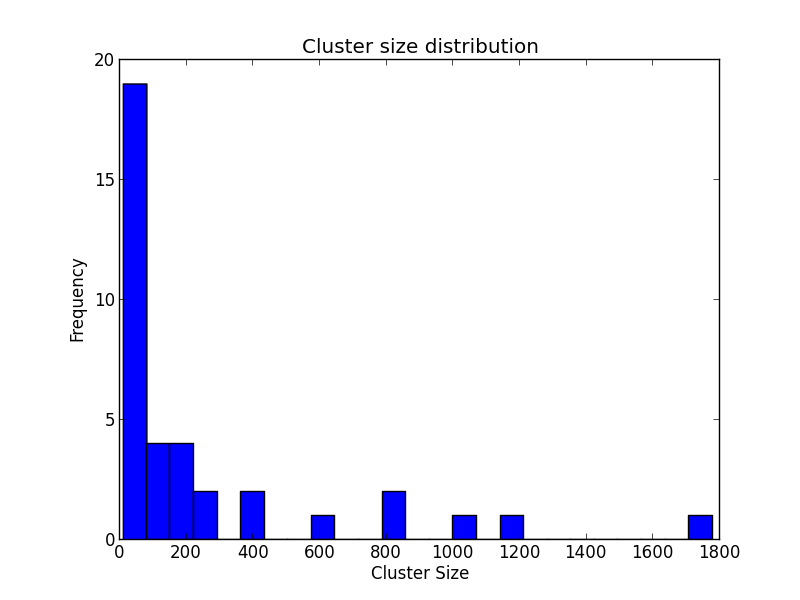
\includegraphics[scale=0.40]{images/cluster_size.png}
\caption{Distribution over cluster sizes for agglomerative clustering. As can be seen there are mainly small clusters with up to 200 words, but there exist also larger clusters.}
\label{cluster_size}
\end{figure}

\subsection{Comparing word context with clusters}
We will define two methods for using the word clusters to define a word relatedness score. In both methods we compare the context of each word with each of the clusters. We define a probability $P( cluster | context )$ for each cluster, and produce a normalized vector $V_p$ of probabilities for each context. The distance between two words is then defined by the cosine similarity between these two vectors.

\subsubsection{Cluster - context intersection}
In the first instance we determine the likelihood of a context being represented by a cluster by counting how many words are in common with the cluster:
\begin{equation} \label{pcc}P( \textit{cluster} | \textit{context}) = \frac{ | \{\textit{cluster} \cap \textit{context}\} |  }{| \textit{cluster} |} \end{equation}
By applying equation \ref{pcc} to all clusters for a given context and normalizing over the different probabilities we get a probability vector $V_{p}$ that defines a mixture of the context over the different clusters. The similarity score for two words is defined by the cosine similarity between the two probability vectors of the two contexts.

\subsubsection{Expanded Cluster - context similarity}
In this method we do not directly compare the words in a cluster with the context, but replace the clusters with the average of the co-occurrence vectors of the words in the cluster. Co-occurrence vectors are extracted from the corpus by finding every instance of a given word and observing the 5 words that occur before and after that word. The co-occurrence vector is a normalized sparse vector that defines the probability for a word co-occurring with a given other word. This extended cluster representation can be compared with a context of a word by cosine similarity of the two vectors. This is how two contexts are compared with every cluster and again cosine similarity can be used to define how related two contexts are.

\section{PALM}
PALM (Probabilistic Agglomeratively-clustered Latent Meanings) is a method for word sense discrimination that simultaneously trains an SVM for every word that can be used for word sense disambiguation. The SVM is able to disambiguate a word by predicting a label best describing the sense of a word when given the probability distribution from the word's expanded context over the agglomeratively-clustered latent meanings (that were obtained using the clustering method described in section \ref{remi}). The predicted labels can for example be used to relabel a corpus before training a recurrent neural network in order to obtain multiple vector representations for one word. 

In this section we describe the PALM method in detail, figure \ref{palmimg} provides an overview of the algorithm. 
\begin{figure*}
\center
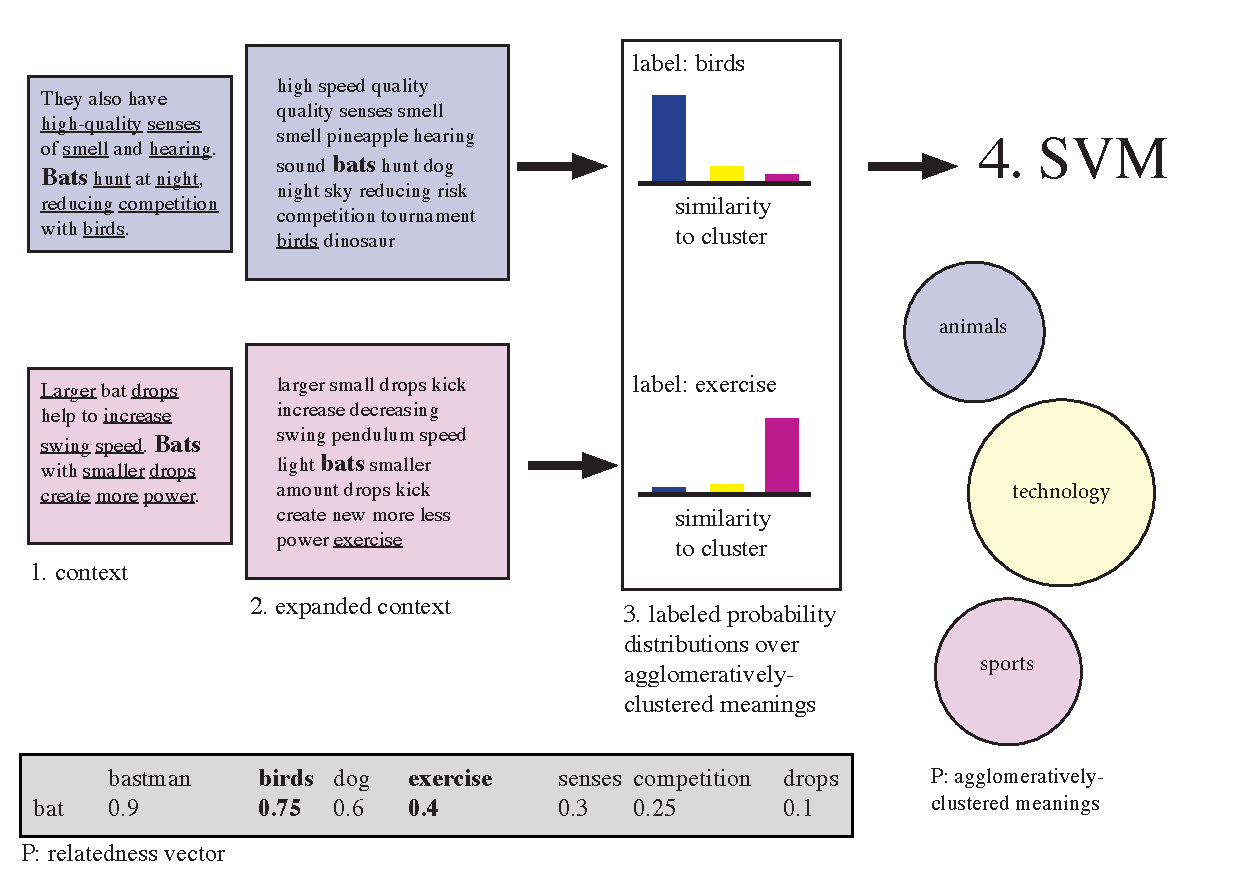
\includegraphics[scale=0.6]{images/palm.pdf}
\caption{The five steps of the PALM algorithm. P: preprocessing, PALM requires agglomeratively-clusterd latent meanings and relatedness vectors for all words in the corpus. 1. Extract every context word $W$ appears in. 2. Expand the context. 3. Choose a label from the expanded context and construct the vector representing the probability distribution from the word's expanded context over the agglomeratively-clustered latent meanings for every context. 4. Train an SVM on these probability distribution vectors using the selected labels.}
\label{palmimg}
\end{figure*}

\subsection{Choosing the label}
Let $W$ be the word for which we want to train the SVM. PALM starts by extracting all contexts from a corpus that $W$ appears in. We define `context' as all words within a window around $W$ (in our experiments we looked five words back and five words ahead). Our aim is to assign a label to each of these contexts that describes the sense of the words best, the collection of labels then represent the different sense a word can have. As we have seen in \cite{analysis} underspecified contexts are often observed. In line with our assumption for the COCONUT baseline (i.e. the co-occurring words that define one meaning of a word are more likely to co-occur with each other than two words that define two different meanings of the word) we expand the context by adding the $n$ (in our experiments we set $n=5$) most related words to every word in the context (except for $W$ itself). Finally, a word $w$ from the expanded context is selected as a label so that:
\begin{equation}\label{label}label = \arg\max_w \frac{r(W, w) + \textit{sim}(W, w)}{2}\end{equation}
where $r(W, w)$ is the relatedness score from equation \ref{r} and $\textit{sim}(W, w)$ denotes the cosine similarity between $W$ and $w$. 


\begin{table}
\center
    \begin{tabular}{lll}
    bat     & course    & bank    \\ \hline
    bird    & need      & invest  \\
    slugger & education & west    \\
    inning  & even      & gaza    \\
    shark   & golf      & foreign \\
    ye      & teach     & central \\
    ~       & learn     & trade   \\
    ~       & have      & fund    \\
    ~       & ~         & finland \\
    \end{tabular}
    \caption{Labels for \textit{bat}, \textit{course} and \textit{bank} after label reduction. The labels are sorted in order of appearance where the top labels are the most frequent and the bottom labels least frequent. }
    \label{labelreduction}
\end{table}

\subsection{Probability distribution over agglomeratively-clustered latent meanings}
Let $P$ be an $N$-dimensional vector describing the probability distribution of a word's context over the clustered meanings. We compute an element $p_i$ in $P$ as follows:
\begin{equation}\label{pa}p_i = \frac{1}{N_c}\sum\limits_{w\in C}sim(w, m_i)\end{equation}
where $N_c$ is the number of contexts, $m_i$ is the vector representation of the $i^{\textit{th}}$ cluster (i.e. latent meaning) and $C$ is the collection of all words in the expanded context. 
Although the values denote the accumulated similarity of the words from the expanded context to the meanings, we can interpret the vector as a probability distribution of a word's context over clustered meanings (when the context and a meaning are very similar, it is very likely that the context imposes this meaning). 

\subsection{Label reduction}
The last step before training the SVM consists of reducing the number of labels. By expanding the context from which the label is selected, we increase the likelihood of selecting the same label multiple times, but many superfluous labels will remain. We apply a modified version of agglomerative clustering on the labels in order to reduce the amount and assure that only `clusters' are formed that represent the same meaning. We have implemented the modified agglomerative clustering method so that it:
\begin{itemize}
\item favors labels that were observed most frequently
\item does not require setting the number of remaining clusters in advance
\end{itemize}
We have implemented a method for label reduction that favors labels that were observed most frequently. We iteratively split the labels into two halves: the upper half (containing labels that were seen most frequently) and the lower half (containing labels that were seen least frequently) and merge a label (and all of its vectors) from the lower half ($w_l$) into a label form the upper half ($w_u$). $w_l$ and $w_u$ are chosen by: 
$$\arg\max_{w_l, w_u} \textit{sim}(w_l, w_u)$$
This process continues until $\textit{sim}(w_l, w_u)$ is below a certain threshold (in our experiments the threshold was $0.5$). Table \ref{labelreduction} shows the remaining labels for the words \textit{bat}, \textit{course} and \textit{bank}.
The reordered labelled data can then be used to train an SVM.

\begin{table*}[t]
    \begin{tabular}{|p{5cm}|p{5cm}|p{2.5cm}|p{1cm}|p{1cm}|}
    \hline
    Word 1                                                                                                                                                                                                      & Word 2                                                                                                                                                                                                      & PALM label1 / label2 / score & Human & SWV  \\ \hline
    In northern New \textbf{Mexico}, the local "black on white" tradition , the Rio Grande white wares, continued well after 1300 AD .                                                           & Women's basketball was added to the Olympics in 1976, which were held in Montreal, Canada with teams such as the Soviet Union, \textbf{Brazil} and Australia rivaling the American squads.  & canada / cup / 0.58          & 0.44  & 0.83 \\ \hline
    It has an aromatic, warm and slightly \textbf{bitter} taste.                                                                                                                                  & AK - a very common beer name in the 1800s - was often referred to as a "mild \textbf{bitter} beer" interpreting "mild" as "unaged".                                                       & taste / war / 0.49           & 0.75  & 1.0  \\ \hline
    Shockley took the lion's share of the \textbf{credit} in public for the invention of transistor, which led to a deterioration of Bardeen's relationship with Shockley .                                         & Payment in kuna, all major \textbf{credit} cards and euros are accepted at all toll gates.                                                                                                                       & invent / pay / 0.48          & 0.31   & 1.0  \\ \hline
    Located downtown along the east \textbf{bank} of the Des Moines River, the plaza is available for parties, social events, movies, concerts, and summer sand volleyball during the warmer months of the year. & This is the basis of all \textbf{money} laundering, a track record of depositing clean money before slipping through dirty money.                                                                                & west / pay / 0.57            & 0.25   & 0.75 \\\hline
    \end{tabular}
    \caption{Four example word pairs from the dataset. For these examples we provide the labels for the two words given by the PALM disambiguation method, including the similarity scores assigned by PALM, SWV and the human annotators. }
    \label{task}
\end{table*}

\section{Experiments}
We evaluate the performance of our WSD methods on the dataset constructed by \cite{global}. The dataset consist of 2003 word pairs and their context. The goal of the task is to assign a similarity measure to all word pairs. 241 word pairs consist of the same word leaving a total of 1712 unique words. Ten human judges assigned similarity scores to all word pairs. Table \ref{task} contains four example word pairs with their context and the scores assigned by two methods and the human annotators. We compute the Spearman correlation between the method's similarity ratings and the average rating of the human annotators. We compare our methods to the Single Word Vector (SWV) baseline that uses only a single word vector for every word and computes the similarity as the cosine similarity between the two words without taking the context into account. \\\\
As mentioned in section \ref{coconut} COCONUT is a method for word sense discrimination. To adapt it for the task of similarity rating, we need a representations of both words in order to compare them. We disambiguated all 1712 words into two different senses ($k = 2$), a sense is represented as a collection of words that indicate this sense. As a representation for the words we choose to use the average word vector of all words that belong to the most appropriate sense of the word given the context, which we define as:
\begin{equation}\label{sense} \arg\max_{\textit{sense}}  | \{\textit{sense} \cap \textit{context}\} |\end{equation}
where \textit{sense} is the set of words in one of the two senses of the disambiguated word and \textit{context} is the set of words in the context.\\\\
To compute the score for PALM we applied the word sense discrimination phase on the \textit{enwiki8} corpus. PALM was able to identify different senses for 1222 of the 1712 unique words of the word pairs, resulting in 1222 SVMs. We then relabeled the 1222 words in the corpus by appending the label predicted by the SVM for the word. To obtain the label, we expand the contexts of both words and use this to compute the probability distribution over the meaning. The trained SVM then provides the label of the word vector that represents the words best in their given contexts. Finally, we used \textit{word2vec} by \cite{word2vec} to obtain 80-dimensional word vectors for all words in the relabeled corpus. For a word pair in the task, we can again obtain the label and use this to find the correct word vector. These word vectors are used to compute the cosine similarity between the two words. Joint PALM is a variation on PALM that computes the similarity between the average word vectors of the single word vector and the word vector selected by PALM.

\begin{table}
\center
    \begin{tabular}{|l|l|l|}
    \hline
    \textbf{WSD Method} & $\rho \times 100$ \\ \hline
    Single Word Vector (SWV) & 60.1 \\ \hline
    COCONUT & 38.2 \\ \hline
    Agglomerative & 19.5 \\ \hline
    Agglomerative + SWV & 60.4 \\ \hline
    Agglomerative Extended & 54.5 \\ \hline
    PALM & 49.9 \\ \hline
    Joint PALM & 57.3 \\ \hline
    \end{tabular}
    \caption{The results}
\end{table}

\section{Conclusion}

\bibliographystyle{acl}
\bibliography{cocobib}

\end{document}
